% Originally: content/week-11.tex, \subsection{The Poincare lemma and simply connected domains} --- promoted

\section{The Poincaré lemma and simply connected domains}
\label{sec:poincare_lemma_simply_connected}

\begin{theorem}[Poincaré Lemma]
\label{thm:poincare_lemma}
Let $U \subseteq \mathbb{R}^n$ be open, and let $\alpha \in \Omega^1(U)$ be a $C^1$ closed $1$-form, that is, $d\alpha = 0$.
Let $\gamma_0, \gamma_1 : [0,1] \to U$ be piecewise $C^1$ paths with the same initial point $x_0$ and the same endpoint $x_1$. Suppose that $\gamma_0$ and $\gamma_1$ are \newterm{homotopic} in $U$ with fixed endpoints. For simplicity, assume that the homotopy $H : [0,1]^2 \to U$ is smooth. Then
\[\int_{\gamma_0} \alpha = \int_{\gamma_1} \alpha.\]
\end{theorem}

\begin{corollary}[Existence of potentials in simply connected domains]
\label{cor:potentials_simply_connected}
Let $U \subseteq \mathbb{R}^n$ be an open \newterm{simply connected} set. Then every closed $C^1$ $1$-form on $U$ is exact. That is, if $\alpha \in \Omega^1(U)$ satisfies $d\alpha = 0$, then there exists a function $f \in C^2(U)$ such that $\alpha = df$.
Equivalently, if $F \in C^1(U, \mathbb{R}^n)$ satisfies the integrability conditions
\[\partial_j F_k = \partial_k F_j \qquad \text{for all } j, k \in \{1,\dots,n\},\]
then $F$ is conservative: there exists a potential $f \in C^2(U)$ such that $\nabla f = F$.
\end{corollary}

\begin{ainote}[Intuition on simply connected spaces]
A space $U$ is simply connected if any closed loop in $U$ can be continuously contracted to a point within $U$ (i.e.\ any two paths with the same endpoints are homotopic). 

% Supplement: Sascha Brack/Class Notes/Week_12_Notes_Monday.pdf, p. 7
\begin{center}
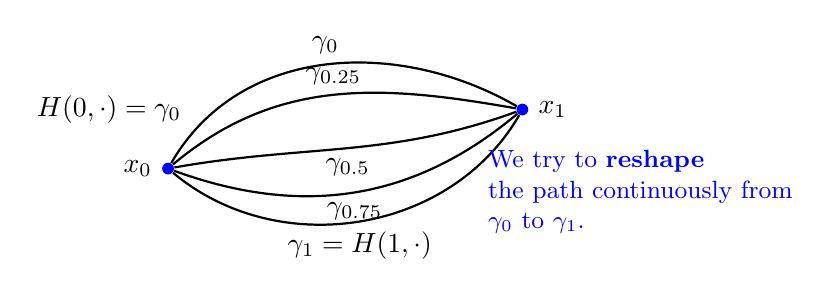
\begin{tikzpicture}[scale=1.5]
  \node[circle, fill=blue, inner sep=1.5pt, label=left:{$x_0$}] (x0) at (0,0) {};
  \node[circle, fill=blue, inner sep=1.5pt, label=right:{$x_1$}] (x1) at (3,0.5) {};
  
  \draw[thick] (x0) to[out=60, in=150] node[pos=0.5, above] {$\gamma_0$} (x1);
  \draw[thick] (x0) to[out=40, in=170] node[pos=0.5, above] {$\gamma_{0.25}$} (x1);
  \draw[thick] (x0) to[out=10, in=200] node[pos=0.5, below] {$\gamma_{0.5}$} (x1);
  \draw[thick] (x0) to[out=-20, in=220] node[pos=0.5, below] {$\gamma_{0.75}$} (x1);
  \draw[thick] (x0) to[out=-40, in=240] node[pos=0.5, below] {$\gamma_1 = H(1,\cdot)$} (x1);
  \node at (-0.5, 0.5) {$H(0,\cdot) = \gamma_0$};
  
  \node[blue, align=left, font=\small] at (4, -0.2) {We try to \textbf{reshape}\\the path continuously from\\$\gamma_0$ to $\gamma_1$.};
\end{tikzpicture}
\end{center}

Examples of simply connected spaces:
\begin{itemize}
    \item $\mathbb{R}^n$
    \item $\mathbb{R}^3 \setminus \{(0,0,0)\}$
\end{itemize}
Examples of spaces that are \emph{not} simply connected:
\begin{itemize}
    \item $S^1 \subseteq \mathbb{R}^2$ (the unit circle)
    \item $\mathbb{R}^3 \setminus \operatorname{span}\{(0,0,1)\transp\}$ (the $z$-axis removed)
    \item The torus
\end{itemize}
This topological property is what allows the integrability conditions to globally imply the existence of a potential.
\end{ainote}

% Supplement: Analysis_II_Script_v1.pdf, p. 153
\begin{example}[Integrability without a potential: why simple connectedness is needed]
\label{ex:vortex_field_not_conservative}
Let $U := \mathbb{R}^2\setminus\{0\}$ (which is \emph{not} simply connected, unlike its
$3$-dimensional analogue $\mathbb{R}^3\setminus\{0\}$ listed above) and
\[F(x,y) := \left(\frac{-y}{x^2+y^2},\ \frac{x}{x^2+y^2}\right), \qquad (x,y) \in U.\]
A direct computation gives
\[\partial_1F_2 = \partial_x\!\left(\frac{x}{x^2+y^2}\right) = \frac{-x^2+y^2}{(x^2+y^2)^2}
  = \partial_y\!\left(\frac{-y}{x^2+y^2}\right) = \partial_2F_1,\]
so $F$ satisfies the integrability conditions (\cref{lem:integrability_conditions})
\emph{everywhere} on $U$. Yet $F$ is not conservative: for the loop
$\gamma(t) := (\cos(2\pi t),\sin(2\pi t))$, $t\in[0,1]$, tracing the unit circle once
counterclockwise,
\[\oint_\gamma F\cdot d\gamma
  = 2\pi\int_0^1\langle(-\sin(2\pi t),\cos(2\pi t)),(-\sin(2\pi t),\cos(2\pi t))\rangle\,dt
  = 2\pi \neq 0,\]
which by \cref{prop:work_difference_potential} is impossible for a conservative field (a closed
loop would have to return $f(\gamma(1))-f(\gamma(0))=0$). This is exactly the witness that
\cref{cor:potentials_simply_connected} needs the hypothesis it has: the integrability
conditions are necessary but, on a domain that is not simply connected, not sufficient.
\end{example}
